\section{B: Hello, World}

\begin{frame}[fragile]
\frametitle{Hello World!}

\begin{columns}
\begin{column}{0.5\textwidth}
\begin{figure}[h]
\centerline{
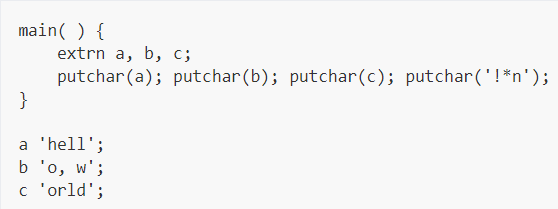
\includegraphics[width=1.0\textwidth]{../Figs/blang2.png}
}
\centerline{
{\tiny Hello World first seen in: Brian Kernighan, {\it A Tutorial Introduction to the Language B}, 1972}
}
\end{figure}
\end{column}

\pause
\begin{column}{0.45\textwidth}
\lstinputlisting[style=basicc]{../Code/ChapB/helloworld.c}
\outputlisting{../Code/ChapB/helloworld.autoout}
\end{column}

\end{columns}
\end{frame}



\begin{frame}[fragile]
\frametitle{Dissecting the 1st Program}

\begin{itemize}[<+->]
\item Comments are bracketed by the {\bf /*} and {\bf */} pair.
\item
\begin{verbatim}
#include <stdio.h>
\end{verbatim}
Lines that begin with a {\bf \#}
are called preprocessing directives.
\item \begin{verbatim}
int main(void)
\end{verbatim}
Every program has a function called {\em main()}

\item Statements are grouped using braces,
\begin{verbatim}
{ ... }
\end{verbatim}

\item \verb+printf()+ One of the pre-defined library functions being called (invoked) using a single argument the string~:
\begin{verbatim}
"Hello, world!\n"
\end{verbatim}
\item The \verb+\n+ means print the single character {\it newline}.
\item Notice all declarations and statements are terminated with a
semi-colon.
\item \verb+return(0)+
Instruct the Operating System that the function
\verb+main()+ has completed successfully.
\end{itemize}
\end{frame}



\begin{frame}[fragile]
\frametitle{Area of a Rectangle}
\begin{columns}

\begin{column}{0.9\textwidth}
\lstinputlisting[style=basicc]{../Code/ChapB/arearect.c}
\outputlisting{../Code/ChapB/arearect.autoout}
\end{column}

\end{columns}
\end{frame}

\begin{frame}[fragile]
\frametitle{Dissecting the Area Program}

\begin{columns}
\begin{column}{0.40\textwidth}
\begin{itemize}[<+->]
\item \verb^//^ One line comment.
\item \verb^#include <stdio.h>^ Always required when using I/O.
\item \verb^int side1, side2, area;^ {\it Declaration}
\item \verb^side2 = 8;^ {\it  Assignment }
\item \verb^printf()^ has 2 Arguments.
The {\it control string}
contains a \verb+%i+ to indicate an integer is to be printed.
\end{itemize}
\end{column}

\pause
\begin{column}{0.55\textwidth}
\begin{lstlisting}[style=basicc]
preprocessing directives

int main(void)
{
   declarations

   statements
}
\end{lstlisting}
\end{column}

\end{columns}
\end{frame}




\begin{frame}[fragile]
\frametitle{Arithmetic Operators}

\begin{itemize}[<+->]
\item \verb^+ , - , / , *, %^
\item Addition, Subtraction, Division, Multiplication,\\ Modulus.
\item Integer arithmetic discards remainder i.e.\\
\verb+1/2+ is 0 , \verb+7/2+ is 3.
\item Modulus (Remainder) Arithmetic.\\
\verb+7%4+ is 3, \verb+12%6+ is 0.

\item
Only available for integer arithmetic.
\end{itemize}
\end{frame}



\begin{frame}[fragile]
\frametitle{The Character Type}

\begin{columns}
\begin{column}{0.55\textwidth}
\lstinputlisting[style=basicc]{../Code/ChapB/chars.c}
\outputlisting{../Code/ChapB/chars.autoout}
\end{column}

\pause
\begin{column}{0.45\textwidth}
\begin{itemize}[<+->]
\item The  keyword \verb+char+ stands for character.
\item Used with single quotes i.e.
\verb^'A'^, or \verb^'+'^.
\item Some keyboards have a second single quote the {\bf back quote} \verb^`^
\item Note the \verb+%c+ conversion format.
\end{itemize}
\end{column}

\end{columns}
\end{frame}


\begin{frame}[fragile]
\frametitle{Floating Types}
\begin{columns}
\begin{column}{0.55\textwidth}
\lstinputlisting[style=basicc]{../Code/ChapB/floats.c}
\outputlisting{../Code/ChapB/floats.autoout}
\end{column}

\pause
\begin{column}{0.45\textwidth}
\begin{itemize}[<+->]
\item In C there are three common floating types~:
    \begin{enumerate}[<+->]
        \item \verb+float+
        \item \verb+double+
        \item \verb+long double+
    \end{enumerate}
\item The {\it Working Type} is doubles.
\end{itemize}
\end{column}

\end{columns}
\end{frame}


\begin{frame}[fragile]
\frametitle{The Preprocessor}

\begin{itemize}[<+->]
\item A \verb+#+ in the first column signifies
a preprocessor statement.

\item \verb+#include <file.h>+
Exchange this line for
the entire contents of \verb+file.h+,
which is to be found in a standard place.

\item \verb+#define PI 3.14159265358979+  Replaces all occurrences of \verb+PI+
with\\ \verb+3.14159265358979+.

\item
Include files generally contain other \verb+#define+'s
and \verb+#include+'s (amongst other things).

\end{itemize}
\end{frame}



\begin{frame}[fragile]
\frametitle{Using printf()}

\begin{itemize}[<+->]
\item \verb+printf( fmt-str, arg1, arg2, ...);+
\end{itemize}

\begin{center}
\begin{tabular}{|c|l|} \hline
\verb+%c+   & Characters \\ \hline
 \verb+%i+  & Integers \\ \hline
 \verb+%e+  & Floats/Doubles (Engineering Notation) \\ \hline
 \verb+%f+  & Floats/Doubles \\ \hline
 \verb+%s+  & Strings \\ \hline
\end{tabular}
\end{center}

\begin{itemize}[<+->]
\item Fixed-width fields: \verb+printf("F:%7f\n", f);+ \\
\verb+F: 3.0001+
\item Fixed Precision: \verb+printf("F:%.2f\n", f);+\\
\verb+F:3.00+
\end{itemize}
\end{frame}



\begin{frame}[fragile]
\frametitle{Using scanf()}
\begin{itemize}[<+->]
\item Similar to \verb+printf()+ but deals with
{\it input} rather than {\it output}.
\item \verb+scanf(fmt-str, &arg1, &arg2, ...);+
\item Note that the {\it address} of the argument is required.
\end{itemize}
\begin{center}
\begin{tabular}{|c|l|} \hline
\verb+%c+   & Characters \\ \hline
\verb+%i+   & Integers \\ \hline
\verb+%f+   & Floats \\ \hline
\verb+%lf+  & Doubles \\ \hline
\verb+%s+   & Strings \\ \hline
\end{tabular}
\end{center}
\begin{itemize}[<+->]
\item Note doubles handled differently than floats.
\end{itemize}
\end{frame}




\begin{frame}[fragile]
\frametitle{While Loops}
\begin{columns}
\begin{column}{0.35\textwidth}
\begin{lstlisting}
while (test is true) {
    statement 1;
        ...
    statement n;
}
\end{lstlisting}
\end{column}

\pause
\begin{column}{0.60\textwidth}
\lstinputlisting[style=basicc]{../Code/ChapB/sums.c}
\outputlisting{../Code/ChapB/sums.manout}
\end{column}
\end{columns}
\end{frame}



\begin{frame}[fragile]
\frametitle{Common Mistakes}

\begin{itemize}[<+->]
\item Missing "
\begin{lstlisting}[style=basicc,numbers=none]
printf("%c\n, ch);
\end{lstlisting}

\item Missing ;
\begin{lstlisting}[style=basicc,numbers=none]
a = a + 1
\end{lstlisting}

\item Missing Address in {\tt scanf()}
\begin{lstlisting}[style=basicc,numbers=none]
scanf("%i", a);
\end{lstlisting}
\end{itemize}
\end{frame}
